\documentclass[aspectratio=169,10pt,xcolor=table]{beamer}
\usetheme{metropolis}
\usepackage[T1]{fontenc}
\usepackage{helvet}
\renewcommand{\familydefault}{\sfdefault}
\usepackage{tikz,booktabs,colortbl}
\usetikzlibrary{arrows.meta, positioning, fit, shapes.geometric, decorations.pathreplacing}

% Slide titles: Arial-like (Helvetica), regular weight, black on white (as LU_Slides). 15 pt: on this 160 mm page 20 pt wraps most titles.
\setbeamercolor{frametitle}{fg=black,bg=white}
\setbeamerfont{frametitle}{size=\fontsize{15}{18}\selectfont,series=\mdseries,family=\sffamily}
\setbeamercolor{title}{fg=black}
\setbeamerfont{title}{size=\fontsize{18}{22}\selectfont,series=\mdseries}

\title{Cholesky in Mixed Precision, Watched by \textsc{NixNan}}
\subtitle{When lowering the precision loses positive definiteness}
\author{Ganesh Gopalakrishnan}
\date{SC26 tutorial}

\tikzset{
  graybox/.style={draw, thick, align=center, font=\scriptsize, fill=gray!10, minimum height=1.1cm},
  bluebox/.style={draw, thick, rounded corners=2pt, align=center, font=\scriptsize, fill=blue!7, minimum height=1.1cm},
  greenbox/.style={draw, thick, rounded corners=2pt, align=center, font=\scriptsize, fill=green!12, minimum height=1.1cm},
  redbox/.style={draw, thick, rounded corners=2pt, align=center, font=\scriptsize, fill=red!12, minimum height=1.1cm},
  orangebox/.style={draw, thick, rounded corners=2pt, align=center, font=\scriptsize, fill=orange!20, minimum height=1.1cm},
  dashbox/.style={draw, thick, dashed, rounded corners=2pt, align=center, font=\scriptsize, fill=white, minimum height=1.1cm},
  flowarrow/.style={-{Stealth[length=2.2mm, width=1.6mm]}, thick},
}
\newcommand{\ok}[1]{\cellcolor{green!15}#1}
\newcommand{\inacc}[1]{\cellcolor{orange!30}#1}
\newcommand{\brk}[1]{\cellcolor{red!25}#1}

\begin{document}
\maketitle

% ------------------------------------------------------------------ 1
\begin{frame}{The question, and what we test}
\small
\begin{itemize}
\item A dense SPD system $Ax=b$: Cholesky $A=LL^T$ is the standard solver, and its trailing update is a GEMM, so it maps well to \textbf{tensor cores}.
\item \textbf{Claim to test:} if the precision is lowered without regard to the condition number, rounding can destroy the small positive Schur-complement
pivot, and the factorization hits $L_{jj}=\sqrt{S_{jj}}$ with $S_{jj}\le 0$: a NaN, or a division by zero.
\item NixNan should locate the exception (kernel, instruction, precision), not merely report that the residual is bad.
\item \textbf{And its opposite:} a bad condition number does not guarantee an exception. Often the answer is finite and wrong.
\end{itemize}
\vspace{2mm}\centering
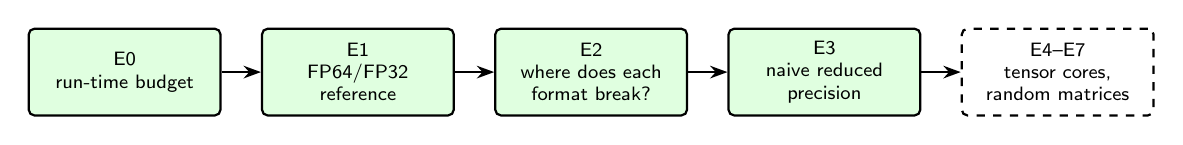
\begin{tikzpicture}[node distance=5mm]
  \node[greenbox, text width=2.2cm] (e0) {E0\\run-time budget};
  \node[greenbox, right=of e0, text width=2.2cm] (e1) {E1\\FP64/FP32 reference};
  \node[greenbox, right=of e1, text width=2.2cm] (e2) {E2\\where does each format break?};
  \node[greenbox, right=of e2, text width=2.2cm] (e3) {E3\\naive reduced precision};
  \node[dashbox, right=of e3, text width=2.2cm] (e4) {E4--E7\\tensor cores, random matrices};
  \foreach \u/\v in {e0/e1,e1/e2,e2/e3,e3/e4} \draw[flowarrow] (\u) -- (\v);
\end{tikzpicture}

{\scriptsize green = done, with logs and tables in this deck; dashed = planned}
\end{frame}

% ------------------------------------------------------------------ 2
\begin{frame}{Algorithm: Cholesky, two code paths}
\footnotesize
$A=LL^T,\quad L_{jj}=\sqrt{S_{jj}},\quad L_{ij}=S_{ij}/L_{jj},\quad S\leftarrow S-L_{:j}L_{:j}^T$ \hfill (no pivoting: SPD guarantees positive pivots)

\vspace{2mm}\centering
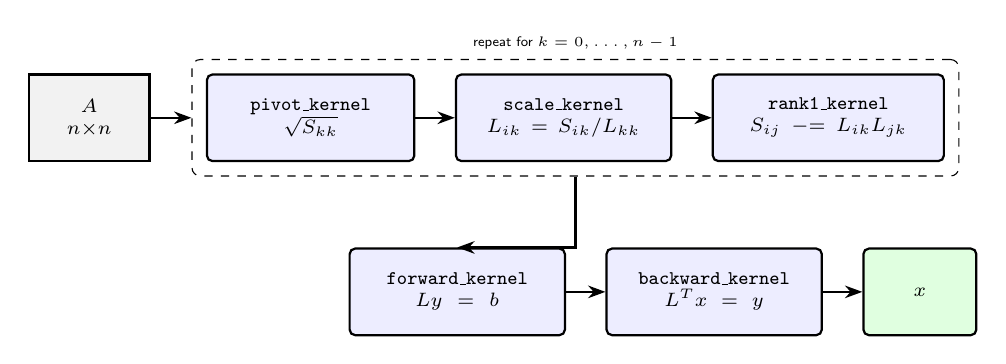
\begin{tikzpicture}[node distance=5mm]
  \node[graybox, text width=1.3cm] (A) {$A$\\$n{\times}n$};
  \node[bluebox, right=7mm of A, text width=2.4cm] (piv) {\texttt{pivot\_kernel}\\$\sqrt{S_{kk}}$};
  \node[bluebox, right=of piv, text width=2.5cm] (sc) {\texttt{scale\_kernel}\\$L_{ik}=S_{ik}/L_{kk}$};
  \node[bluebox, right=of sc, text width=2.7cm] (r1) {\texttt{rank1\_kernel}\\$S_{ij}\mathrel{-}=L_{ik}L_{jk}$};
  \node[draw, dashed, rounded corners=3pt, fit=(piv)(sc)(r1), inner sep=5pt, label={[font=\tiny]above:repeat for $k=0,\dots,n-1$}] (loop) {};
  \node[bluebox, below=9mm of loop, text width=2.5cm, xshift=-1.5cm] (fw) {\texttt{forward\_kernel}\\$Ly=b$};
  \node[bluebox, right=of fw, text width=2.5cm] (bw) {\texttt{backward\_kernel}\\$L^Tx=y$};
  \node[greenbox, right=of bw, text width=1.2cm] (x) {$x$};
  \draw[flowarrow] (A) -- (loop.west |- A.east); \draw[flowarrow] (piv) -- (sc); \draw[flowarrow] (sc) -- (r1);
  \draw[flowarrow] (loop.south) -- (loop.south |- fw.north) -- (fw.north);
  \draw[flowarrow] (fw) -- (bw); \draw[flowarrow] (bw) -- (x);
\end{tikzpicture}

\vspace{3mm}\raggedright
\begin{tabular}{p{0.46\textwidth}p{0.46\textwidth}}
\textbf{unblocked:} 3 launches per column, 5 distinct kernels.&
\textbf{blocked} ($NB{=}32$): \texttt{potrf\_tile} (diagonal tile), \texttt{trsm\_panel}, \texttt{syrk} (trailing update; the tensor-core slot in E4), same two solves.\\
\end{tabular}

\vspace{2mm}
{\scriptsize Pivot errors are only \emph{recorded} (\texttt{atomicMin}); the arithmetic continues, so a bad pivot becomes Inf/NaN exactly as in unguarded code.}
\end{frame}

% ------------------------------------------------------------------ 3
\begin{frame}{The test matrix: $A_\delta = \mathbf{1}\mathbf{1}^T+\delta I$}
\small
\begin{columns}[T]\begin{column}{0.5\textwidth}
\begin{itemize}
\item SPD for every $\delta>0$: eigenvalues $n+\delta$ (once) and $\delta$ ($n{-}1$ times).
\item $\kappa_2=(n+\delta)/\delta\approx n/\delta$. Checked against the eigenvalues of the stored matrix.
\item If storage rounds $1+\delta\mapsto 1$, the stored matrix is $\mathbf{1}\mathbf{1}^T$: \textbf{rank one, not SPD}. Second pivot $=0$.
\end{itemize}
\vspace{2mm}
\begin{tabular}{llr}
\toprule
 & $\delta$ & $\kappa_2$ ($n{=}256$)\\
\midrule
M0 & $2^{-6}$ & $1.6\times10^{4}$\\
M1 & $2^{-12}$ & $1.0\times10^{6}$\\
\bottomrule
\end{tabular}
\end{column}\begin{column}{0.48\textwidth}
\centering
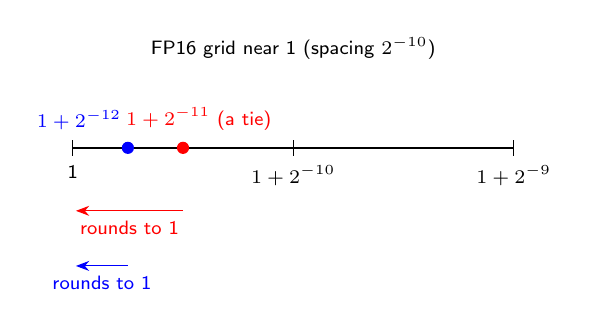
\begin{tikzpicture}[x=0.8cm,y=1cm,font=\scriptsize]
  \draw[thick] (0,0) -- (7,0);
  \foreach \x/\l in {0/1, 3.5/{$1+2^{-10}$}, 7/{$1+2^{-9}$}} {\draw (\x,-0.1) -- (\x,0.1); \node[below] at (\x,-0.1) {\l};}
  \node[above, text width=5.5cm, align=center] at (3.5,1.0) {FP16 grid near 1 (spacing $2^{-10}$)};
  \fill[red] (1.75,0) circle (2.2pt); \node[red, above] at (2.0,0.1) {$1+2^{-11}$ (a tie)};
  \fill[blue] (0.875,0) circle (2.2pt); \node[blue, above] at (0.1,0.1) {$1+2^{-12}$};
  \draw[red, -{Stealth}] (1.75,-0.8) -- (0.05,-0.8) node[midway, below] {rounds to 1};
  \draw[blue, -{Stealth}] (0.875,-1.5) -- (0.05,-1.5) node[midway, below] {rounds to 1};
\end{tikzpicture}

\vspace{2mm}
\begin{tabular}{lll}
\toprule
format & mantissa bits & $\delta$ lost from\\
\midrule
BF16 & 7 & $2^{-8}$\\
FP16 & 10 & $2^{-11}$\\
TF32 & 10 & $2^{-12}$ (ties away)\\
FP32 & 23 & $2^{-24}$\\
\bottomrule
\end{tabular}
\end{column}\end{columns}
\end{frame}

% ------------------------------------------------------------------ 4
\begin{frame}{NixNan set-up for this study}
\scriptsize
\begin{columns}[T]\begin{column}{0.54\textwidth}
\begin{tabular}{@{}p{3.3cm}p{3.7cm}@{}}
\toprule
\texttt{LD\_PRELOAD=nixnan.so} & instruments every kernel, report at exit\\
\texttt{TIME\_KERNELS=1} & per-kernel time: first launch $\approx$0.3 s\\
\texttt{PRINT\_ILL\_INSTR=1} & print each exception with its SASS\\
\texttt{ENABLE\_FUN\_DETAIL=1} & kernel name on every line\\
\texttt{LINE\_INFO} (default on) & \texttt{file:line}, where available\\
\texttt{NIXNAN\_TIMEOUT} & self-terminate after $N$ s\\
\bottomrule
\end{tabular}

\vspace{3mm}
\normalsize\textbf{Cost:} 5 kernels $\Rightarrow$ \textbf{3 s} under nixnan (0.3 s native); $n{=}64$: 2.2 s.\\[1mm]
\footnotesize The library-based \texttt{mpir\_gpu/ir\_gpu} (cuSOLVER/cuBLAS) takes \textbf{88 s}. Custom kernels keep every run inside the 2-minute budget.
\end{column}\begin{column}{0.42\textwidth}
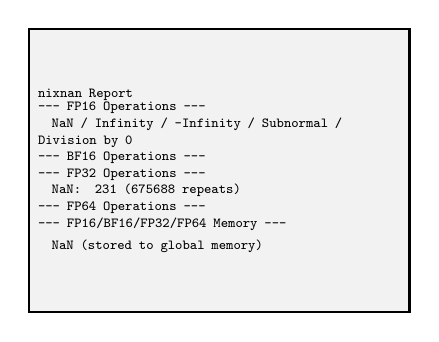
\begin{tikzpicture}[font=\scriptsize]
  \node[graybox, text width=4.6cm, align=left, minimum height=3.6cm, anchor=north west] at (0,0) {%
   \ttfamily\tiny
   nixnan Report\\[-1pt]
   --- FP16 Operations ---\\
   \ \ NaN / Infinity / -Infinity / Subnormal / Division by 0\\
   --- BF16 Operations ---\\
   --- FP32 Operations ---\\
   \ \ NaN:\ \ 231 (675688 repeats)\\
   --- FP64 Operations ---\\
   --- FP16/BF16/FP32/FP64 Memory ---\\
   \ \ NaN (stored to global memory)};
\end{tikzpicture}

\vspace{1mm}{\footnotesize Each counter: \textbf{unique sites (repeats)}. One section per precision, memory sections count NaN only.}
\end{column}\end{columns}
\end{frame}

% ------------------------------------------------------------------ 5
\begin{frame}{E1: reference; NixNan is silent}
\centering\scriptsize
\begin{tabular}{llrrrr}
\toprule
 & & \multicolumn{2}{c}{M0 ($\kappa_2=1.6\times10^{4}$)} & \multicolumn{2}{c}{M1 ($\kappa_2=1.0\times10^{6}$)}\\
arithmetic & path & $\|A-LL^T\|/\|A\|$ & $\|x-1\|/\|1\|$ & $\|A-LL^T\|/\|A\|$ & $\|x-1\|/\|1\|$\\
\midrule
F64 & unblocked & $1.0\!\times\!10^{-16}$ & $1.1\!\times\!10^{-14}$ & $1.1\!\times\!10^{-16}$ & $3.1\!\times\!10^{-13}$\\
F64 & blocked & $9.5\!\times\!10^{-17}$ & $4.0\!\times\!10^{-13}$ & $1.1\!\times\!10^{-16}$ & $3.3\!\times\!10^{-13}$\\
F32 & unblocked & $1.3\!\times\!10^{-9}$ & $8.8\!\times\!10^{-6}$ & $1.3\!\times\!10^{-9}$ & $7.5\!\times\!10^{-6}$\\
F32 & blocked & $1.0\!\times\!10^{-7}$ & $5.6\!\times\!10^{-4}$ & $5.2\!\times\!10^{-8}$ & $1.8\!\times\!10^{-2}$\\
\bottomrule
\end{tabular}


\vspace{3mm}\small
\fcolorbox{black}{green!12}{\parbox{0.88\textwidth}{\centering All 8 runs: status ok, no bad pivot, \textbf{no nixnan exception} in any precision or in memory.\\
The matrix is valid and the kernels are right, so every later failure is due to precision.}}

\vspace{2mm}\footnotesize\raggedright
\begin{itemize}
\item In FP32 the \emph{forward} error depends on the code path (M1: $7.5\times10^{-6}$ unblocked, $1.8\times10^{-2}$ blocked) although both factorizations are accurate: forward error is the sensitive metric.
\end{itemize}
\end{frame}

% ------------------------------------------------------------------ 6
\begin{frame}{E2: where does each format break?}
\centering
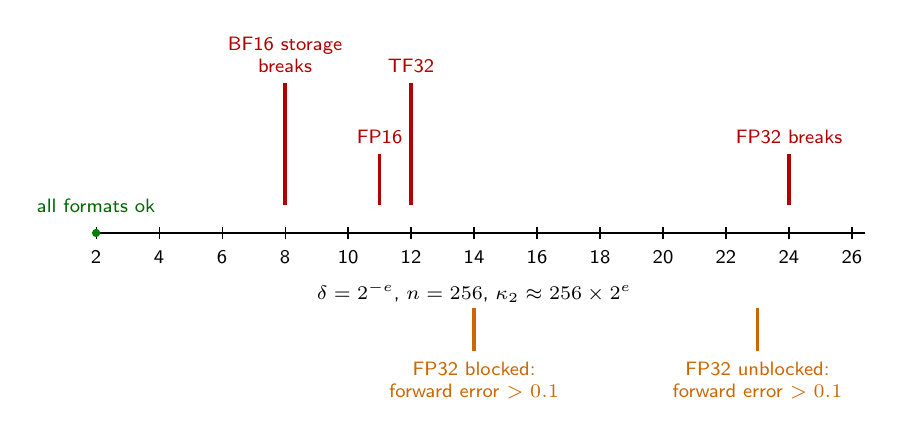
\begin{tikzpicture}[x=0.40cm,y=1cm,font=\scriptsize]
  \draw[thick] (2,0) -- (26.4,0);
  \foreach \e in {2,4,...,26} {\draw (\e,-0.08) -- (\e,0.08); \node[below] at (\e,-0.1) {\e};}
  \node[below] at (14,-0.5) {$\delta=2^{-e}$, $n=256$, $\kappa_2\approx 256\times2^{e}$};
  \draw[red!70!black, very thick] (8,0.35) -- (8,1.9) node[above, text width=1.7cm, align=center] {BF16 storage breaks};
  \draw[red!70!black, very thick] (11,0.35) -- (11,1.0) node[above, text width=1.7cm, align=center] {FP16};
  \draw[red!70!black, very thick] (12,0.35) -- (12,1.9) node[above, text width=1.7cm, align=center] {TF32};
  \draw[orange!80!black, very thick] (14,-0.95) -- (14,-1.5) node[below, text width=2.2cm, align=center] {FP32 blocked: forward error $>0.1$};
  \draw[orange!80!black, very thick] (23,-0.95) -- (23,-1.5) node[below, text width=2.2cm, align=center] {FP32 unblocked: forward error $>0.1$};
  \draw[red!70!black, very thick] (24,0.35) -- (24,1.0) node[above, text width=1.7cm, align=center] {FP32 breaks};
  \fill[green!50!black] (2,0) circle (1.5pt) node[above=4pt, text=green!40!black] {all formats ok};
\end{tikzpicture}

\vspace{1mm}\scriptsize
\begin{itemize}
\item \textbf{Storage breakdown} at the format's grid: the stored matrix becomes $\mathbf{1}\mathbf{1}^T$; first bad pivot is \textbf{index 1} in every case. FP16/BF16: ties round to even; TF32 (\texttt{cvt.rna}) rounds the tie up, so it survives one step longer.
\item \textbf{Demo point $\delta=2^{-12}$ (M1):} FP32 is ok; TF32, FP16 and BF16 all break. At $\delta=2^{-10}$ FP16/TF32 still work, BF16 breaks.
\item FP64 breaks at $e=53$ (matrix itself), with forward error $>0.1$ from $e=43/52$.
\end{itemize}
\end{frame}

% ------------------------------------------------------------------ 7
\begin{frame}{E3a: FP16 storage, $\delta=2^{-12}$: the chain}
\footnotesize
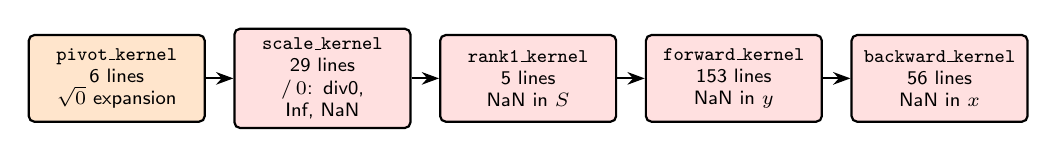
\begin{tikzpicture}[node distance=3.5mm]
  \node[orangebox, text width=2.0cm] (a) {\texttt{pivot\_kernel}\\6 lines\\$\sqrt{0}$ expansion};
  \node[redbox, right=of a, text width=2.0cm] (b) {\texttt{scale\_kernel}\\29 lines\\$/\,0$: div0, Inf, NaN};
  \node[redbox, right=of b, text width=2.0cm] (c) {\texttt{rank1\_kernel}\\5 lines\\NaN in $S$};
  \node[redbox, right=of c, text width=2.0cm] (d) {\texttt{forward\_kernel}\\153 lines\\NaN in $y$};
  \node[redbox, right=of d, text width=2.0cm] (e) {\texttt{backward\_kernel}\\56 lines\\NaN in $x$};
  \foreach \u/\v in {a/b,b/c,c/d,d/e} \draw[flowarrow] (\u) -- (\v);
\end{tikzpicture}

\vspace{3mm}
\begin{columns}[T]\begin{column}{0.52\textwidth}
\textbf{nixnan report (FP32 section only):}\\[1mm]
\begin{tabular}{lrr}
\toprule
counter & unique & repeats\\
\midrule
NaN & 231 & 675\,688\\
Infinity & 13 & 28\\
Division by 0 & 4 & 11\\
memory NaN (STG) & 1 & 94\,655\\
\bottomrule
\end{tabular}

\vspace{2mm}
BF16 storage: identical counts. Blocked path: NaN 566, Inf 17, Div0 5.
\end{column}\begin{column}{0.44\textwidth}
\begin{itemize}
\item Stored matrix $=\mathbf{1}\mathbf{1}^T$, second pivot exactly 0 (\textbf{bad pivot = 1}).
\item $L_{i1}=1$ for all $i$; the update gives $S=0$; $\sqrt0=0$; then $0/0$.
\item NaNs travel through the update and both substitutions to the output.
\item All exceptions are FP32: the narrow-format rounding is on the host, and conversions are not instrumented.
\end{itemize}
\end{column}\end{columns}
\end{frame}

% ------------------------------------------------------------------ 8
\begin{frame}[fragile]{The first report is not the defect}
\scriptsize
\fcolorbox{black}{gray!10}{\parbox{0.95\textwidth}{\ttfamily
error [div0]     operand 1 of MUFU.RSQ R7, R0     in pivot\_kernel \ \ \ of type f32\\
error [infinity] operand 0 of MUFU.RSQ R7, R0     in pivot\_kernel \ \ \ of type f32\\
error [div0]     operand 1 of MUFU.RCP R2, R7     in scale\_kernel \ \ \ of type f32\\
error [infinity] operand 0 of MUFU.RCP R2, R7     in scale\_kernel \ \ \ of type f32\\
error [NaN]      operand 0 of FFMA R3, -R7, R2, 1 in scale\_kernel \ \ \ of type f32}}

\vspace{3mm}\footnotesize
\begin{itemize}
\item \texttt{sqrt(0)} is compiled to a \texttt{MUFU.RSQ} expansion. \texttt{rsqrt(0)=Inf} inside it is flagged, yet the final result $0$ is \textbf{correct}.
\item The \textbf{first real failure} is the next kernel: \texttt{MUFU.RCP} of the zero pivot in \texttt{scale\_kernel} (operand 1 is the zero input, operand 0 the Inf result), then NaN from the \texttt{FFMA} fix-up.
\item Same lesson as the \texttt{FFMA}-as-register-move artifact in the LU study: a SASS-level detector reports what the compiled code does. \textbf{Separate the library expansion from the operation that matters.}
\item \texttt{file:line} appears only for the substitution kernels; for \texttt{pivot}, \texttt{scale}, \texttt{rank1} the report has the kernel and the SASS but no source line (cause not found; the cubin has a line table).
\end{itemize}
\end{frame}

% ------------------------------------------------------------------ 9
\begin{frame}{E3b: true FP16/BF16 arithmetic}
\footnotesize
\begin{columns}[T]\begin{column}{0.5\textwidth}
SASS of the FP16 build (\texttt{cuobjdump -sass}):

\vspace{1mm}
\begin{tabular}{lr}
\toprule
instruction & count\\
\midrule
\texttt{HFMA2} (update, solves) & 39\\
\texttt{MUFU.RCP} (division) & 3\\
\texttt{MUFU.SQRT} & 1\\
\texttt{FFMA}, \texttt{FMUL} & 6, 3\\
\texttt{F2FP.PACK\_AB} (convert) & 7\\
\bottomrule
\end{tabular}

\vspace{2mm}
The update is a genuine FP16 fused multiply-add, but \texttt{\_\_hdiv} and \texttt{hsqrt} run in \textbf{FP32} (reciprocal, then convert back).
\end{column}\begin{column}{0.48\textwidth}
\textbf{nixnan at $\delta=2^{-12}$ (breakdown):}\\[1mm]
\begin{tabular}{lrr}
\toprule
section & NaN & Inf, Div0\\
\midrule
FP16 (\texttt{HFMA2}) & 156 (636\,986) & --\\
FP32 (\texttt{MUFU.RCP}\ldots) & 17 (8\,684) & 6, 3\\
\bottomrule
\end{tabular}

\vspace{1mm}
BF16 arithmetic: BF16 NaN 156 (636\,986), FP32 NaN 73, Inf 12, Div0 3.

\vspace{2mm}
The first report is \texttt{MUFU.RCP} in \texttt{scale\_kernel}; the FP16/BF16 NaNs come from the \texttt{HFMA2} updates and substitutions that follow.
\end{column}\end{columns}

\vspace{3mm}\centering
\fcolorbox{black}{blue!7}{\parbox{0.85\textwidth}{\centering To read a half-precision run, look at \textbf{both} the FP16/BF16 and the FP32 sections.}}
\end{frame}

% ------------------------------------------------------------------ 10
\begin{frame}{The silent failure: finite, wrong, and no exception}
\footnotesize\centering
\textbf{FP16 arithmetic}, sweep of $\delta=2^{-e}$\\[1mm]
\scriptsize\begin{tabular}{lccccccccccccc}
\toprule
$e$ & 2 & 3 & 4 & 5 & 6 & 7 & 8 & 9 & 10 & 11 & 12 & 13 & 14\\
\midrule
status & \cellcolor{green!15}ok & \cellcolor{green!15}ok & \cellcolor{green!15}ok & \cellcolor{green!15}ok & \cellcolor{green!15}ok & \cellcolor{green!15}ok & \cellcolor{green!15}ok & \cellcolor{green!15}ok & \cellcolor{orange!30}inacc & \cellcolor{red!25}BRK & \cellcolor{red!25}BRK & \cellcolor{red!25}BRK & \cellcolor{red!25}BRK\\
\bottomrule
\end{tabular}


\vspace{2mm}\footnotesize\textbf{BF16 arithmetic}\\[1mm]
\scriptsize\begin{tabular}{lccccccccccccc}
\toprule
$e$ & 2 & 3 & 4 & 5 & 6 & 7 & 8 & 9 & 10 & 11 & 12 & 13 & 14\\
\midrule
status & \cellcolor{orange!30}inacc & \cellcolor{orange!30}inacc & \cellcolor{orange!30}inacc & \cellcolor{orange!30}inacc & \cellcolor{orange!30}inacc & \cellcolor{orange!30}inacc & \cellcolor{red!25}BRK & \cellcolor{red!25}BRK & \cellcolor{red!25}BRK & \cellcolor{red!25}BRK & \cellcolor{red!25}BRK & \cellcolor{red!25}BRK & \cellcolor{red!25}BRK\\
\bottomrule
\end{tabular}


\vspace{3mm}
\begin{tabular}{llll}
\toprule
arithmetic, $\delta$ & factorization error & forward error $\|x-1\|/\|1\|$ & nixnan\\
\midrule
FP16, $2^{-10}$ ($\kappa_2=2.6\times10^{5}$) & $3.8\times10^{-6}$ & \cellcolor{red!25}$16$ & no exceptions\\
BF16, $2^{-7}$ ($\kappa_2=3.3\times10^{4}$) & $3.1\times10^{-5}$ & \cellcolor{red!25}$16$ & no exceptions\\
\bottomrule
\end{tabular}

\vspace{2mm}\footnotesize\raggedright
\begin{itemize}
\item Small backward error, huge forward error: $\kappa\cdot u\gg1$. The stored matrix is exact, no pivot is $\le0$, so nothing is raised.
\item (BF16's ``inacc'' for $e\le7$ is partly my 0.1 forward-error threshold: BF16 arithmetic is never accurate on this matrix.)
\end{itemize}
\end{frame}

% ------------------------------------------------------------------ 11
\begin{frame}{What each check can see}
\centering\small
\begin{tabular}{lcc}
\toprule
 & silent case (finite, wrong) & breakdown (pivot $\le0$)\\
\midrule
NixNan (NaN / Inf / div-by-zero) & \cellcolor{red!25}blind & \cellcolor{green!15}finds it: kernel, instruction, precision\\
Forward error or residual & \cellcolor{green!15}finds it & \cellcolor{green!15}NaN: finds it\\
Pivot / condition check before dividing & \cellcolor{green!15}finds it, before the solve & \cellcolor{green!15}finds it, before the solve\\
\bottomrule
\end{tabular}

\vspace{5mm}
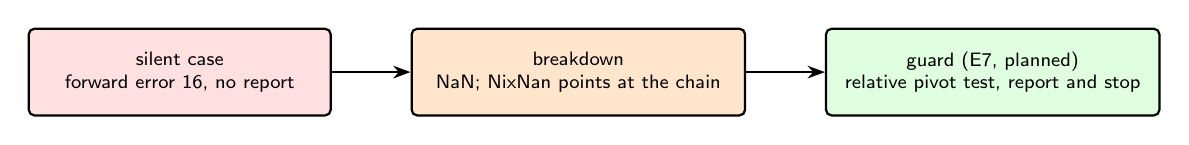
\begin{tikzpicture}[node distance=10mm]
  \node[redbox, text width=3.6cm] (v1) {silent case\\forward error 16, no report};
  \node[orangebox, right=of v1, text width=4.0cm] (v2) {breakdown\\NaN; NixNan points at the chain};
  \node[greenbox, right=of v2, text width=4.0cm] (v3) {guard (E7, planned)\\relative pivot test, report and stop};
  \draw[flowarrow] (v1) -- (v2); \draw[flowarrow] (v2) -- (v3);
\end{tikzpicture}

\vspace{4mm}\footnotesize\raggedright
\begin{itemize}
\item NixNan finds \emph{exceptions}, not ill-conditioning. Pair it with an error check.
\item Same lesson as the LU $\epsilon$-clamp study: a relative check that reports an error beats a silent fix-up.
\end{itemize}
\end{frame}

% ------------------------------------------------------------------ 12
\begin{frame}{Caveats}
\small
\begin{itemize}
\item \textbf{$A_\delta$ is special} (rank one plus a shift): it shows how the failure looks, not how often it happens. Randomised matrices (E5) are the real test.
\item \textbf{FP32 accuracy thresholds depend on the implementation:} LAPACK \texttt{spotrf} reports ``not positive definite'' at $e=16$--22 where our kernels do not; the storage breakdown (e.g.\ FP16 at $e=11$) agrees exactly.
\item Narrow formats are \textbf{emulated by host rounding}; the tensor-core path (device conversion, WMMA inputs) is E4.
\item The ``inaccurate'' status uses my threshold (forward error $>0.1$); it moves the \textit{inacc} boundary, not the breakdown one.
\item TF32's threshold depends on the rounding mode of the tensor-core inputs (ties away vs. to even).
\item One GPU (RTX 3090, sm\_86, CUDA 12.4); nixnan counts reflect how the compiler expands division and square root on this machine.
\end{itemize}
\end{frame}

% ------------------------------------------------------------------ 13
\begin{frame}{Next: tensor cores, random matrices, a guard}
\small\centering
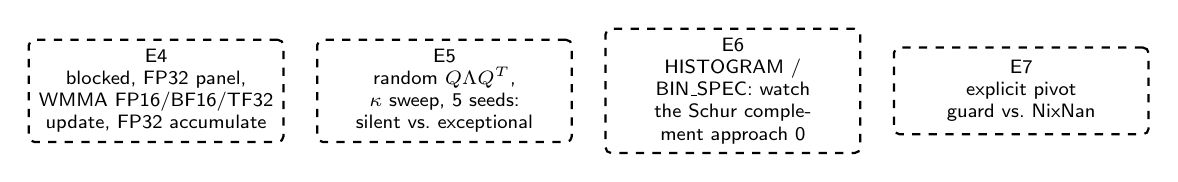
\begin{tikzpicture}[node distance=4mm]
  \node[dashbox, text width=3.0cm] (e4) {E4\\blocked, FP32 panel, WMMA FP16/BF16/TF32 update, FP32 accumulate};
  \node[dashbox, right=of e4, text width=3.0cm] (e5) {E5\\random $Q\Lambda Q^T$, $\kappa$ sweep, 5 seeds: silent vs.\ exceptional};
  \node[dashbox, right=of e5, text width=3.0cm] (e6) {E6\\HISTOGRAM / BIN\_SPEC: watch the Schur complement approach 0};
  \node[dashbox, right=of e6, text width=3.0cm] (e7) {E7\\explicit pivot guard vs.\ NixNan};
\end{tikzpicture}

\vspace{5mm}\raggedright\small
\begin{itemize}
\item E4 checks that the trailing update compiles to \texttt{HMMA.16816.F32} (\texttt{.F32.BF16}, \texttt{HMMA.1684.F32.TF32}) and relates the first exception to the block step $k$.
\item E6 reuses the exponent-binade view from the LU study as a ``danger zone'' monitor.
\item Every run stays within the budget: 1 minute native, 2 minutes with nixnan.
\end{itemize}
\vfill\centering{\footnotesize Reproduce: \texttt{./run\_chol\_story.sh} \quad Full details: \texttt{chol\_report.pdf} \quad Plan and results: \texttt{EXPERIMENT\_PLAN.md}}
\end{frame}

\end{document}
